%%This is a very basic article template.
%%There is just one section and two subsections.

\documentclass[a4paper,11pt,oneside,brazilian]{article}

\usepackage[utf8]{inputenx}
\usepackage[brazilian]{babel}
\usepackage{graphicx}
\usepackage{float}
\usepackage{textgreek}
\usepackage{mathtools}

 
\graphicspath{{../figs/}}
\DeclareGraphicsExtensions{.pdf,.png,.jpg}

\newcommand{\cpar}[2]{\frac{\partial #1}{\partial #2}}
\newcommand{\cspar}[2]{\frac{\partial^2 #1}{\partial #2^2}}
\newcommand{\euTwo}[2]{\sqrt{\left ( #1 \right )^2 + \left ( #2 \right )^2 +
1^2}}
\newcommand{\euThree}[3]{\sqrt{\left ( #1 \right )^2 + \left ( #2 \right
)^2 + \left ( #3 \right )^2 }}



\begin{document}


\section{3-D Reconstruction}

\subsection{Sidescan Sonar}
\label{sonar}

A forma como o \textit{Sidescan} trabalha com o som é análoga a que um
\textit{scanner} usa a luz para capturar uma imagem. Isso permite o uso de
técnicas de simulação ótica como \textit{ray-trace} ou simplificações da propagação
do onda para a geração de imagens de \emph{SONAR}.

Grande parte das diferenças reside na diferença de velocidade entre o som e a
luz. Fazendo ser possível facilmente calcular diferenças de distâncias à partir
das diferenças dos tempos de chegada, mas necessitando tem um tempo não
desprezível de espera para o retorno de uma ensonificação, em contraste com a
iluminação.

De qualquer forma a equação que rege a propagação do som na água é identica à da
luz:

\[\cspar{p}{x} + \cspar{p}{y} + \cspar{p}{z} - \frac{1}{c^2}\cspar{p}{t} = -
\delta(x-x_s,y-y_s,z-z_s)s(t)\]

A equação diferencial permite o uso de métodos numéricos como \emph{diferenças
finitas}, \emph{elementos finitos} e \emph{elementos de contorno}. Entretanto,
nenhum desses se mostra computacionalmente eficiente para frequencias acima de
alguns kilohertz[original].

Como forma de reduzir o esforço computacional, pode-se utilizar um a
simplificação de uma reflexão puramente difusa, i.e. reflectância perfeitamente
\emph{Lambertiana}, a equação para a intensidade de cada píxel da imagem
gerada pelo \emph{SONAR} pode descrita por:

\begin{align}
	I(\textbf{r}) &=  K \Phi(\textbf{r}) R(\textbf{r}) \hat{\textbf{n}} \cdot
\hat{\textbf{r}} \nonumber \\
	&= K \Phi(\textbf{r}) R(\textbf{r}) \cos(\theta(\textbf{r}))
	\label{eq:power}
\end{align}

Onde \textbf{r} é o vetor da origem da ensonificação até o ponto da superfície
que foi ensonificada e \textbf{n} o vetor normal da superfície nesse ponto,
\(I(\textbf{r})\) é a intensidade sonora retornada, \(\Phi(\textbf{r})\) é a
intensidade emitida para um certo ponto, \(R(\textbf{r})\) a reflectância do
ponto e \(K\) uma constante normalizadora. A imagem \ref{fig:sidesgeo} ajuda a
compretender como essa relação será aplicada ao \emph{SONAR}.

Outra consideração é a superfície ser uma função do plano \(X \times
Y\), i.e. ser monovalorado. O que permitirá utilizar algorítimos de otimização
para se encontrar \(Z(x,y)\). É importante ressaltar também que o decaimento
pelo espalhamento da onda não aparece na equação, pois como diversos \emph{SONAR}'s
utilizam um ganho variavel para compensar essa perda ele pode ser deixaido de
lado.

 \begin{figure}[ht]
    \centering
    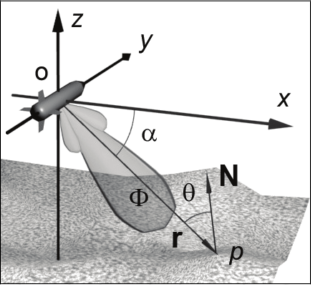
\includegraphics[width=0.4\columnwidth]{sides_geo}
    \caption{Geometria utilizada em [original] para reconstrução.} 
    \label{fig:sidesgeo}
\end{figure}

\subsection{Otimização e Reconstrução}
\subsubsection{Funcional \(I[R,Z,\Phi]\)}
Agora que temos uma descrição para intensidade da onda refletida pelo solo
quando recebida pelo \emph{SONAR} podemos fazer o caminho inverso e tentar
recriar o solo à partir das intensidades.

Seguindo o sistema de coordenadas exposto na imagem \ref{fig:sidesgeo}
definimos:

\begin{align}
&\textbf{r} = (x,0,Z(x,y)) \label{eq:r} \\ 
&\textbf{n} = \left ( -\cpar{Z}{x}(x,y), - \cpar{Z}{y}(x,y),1 \right )
\label{eq:n}
\end{align}

Ao inserir as equações \eqref{eq:r} e \eqref{eq:n} na \eqref{eq:power} obtemos
uma função \(I(x,y)\) que é um funcional \(I[R,Z,\Phi]\) ou seja, dada a função
dos parâmetros podemos calcular a intensidade a intesidade refletida por
qualquer ponto \textbf{p}.

\subsubsection{Mínimos quadrados}

A subdeterminação do problema de resconstrução, onde para cada ponto \textbf{p}
onde se observa a insidade \emph{I} existem três parâmetros a serem estimados,
nomeadamente \emph{R, Z} e \textPhi , nos leva ao uso de algorítmos de
otimização para encontrar valores para os parâmetros. A solução se faz por
mínimos quadrados \emph{E} do erro entre o \textbf{valor medido} pelo sonar em
determinado ponto e o valor calculado da maneira exposta na seção \ref{sonar}
no mesmo ponto (utilizando como base a \eqref{eq:power}):

\[
E = \sum_{x,y}^{} E(x,y) = \sum_{x,y}^{} \left( \hat{I}(x,y) - I(x,y)\right)^2
\]


Assim o problema de otimização pode ser escrito como:

\[
(Z,R,\Phi) = \arg\min(E)
\]


\section{SAS}

\subsection{Introdução}
SAS (Synthetic Aperture Sonar, Sonar de abertura sintética, em tradução livre)
se diferencia dos sonares clássicos pela estrutura da sua abertura. O objetivo
dessa alteração é combinar a resposta de diversos \emph{pings}, emissões do
\emph{sonar}, para aumentar a resolução, podendo chegar a resolução de
\cite{Hansen2011a}.

 \begin{figure}[ht]
    \centering
    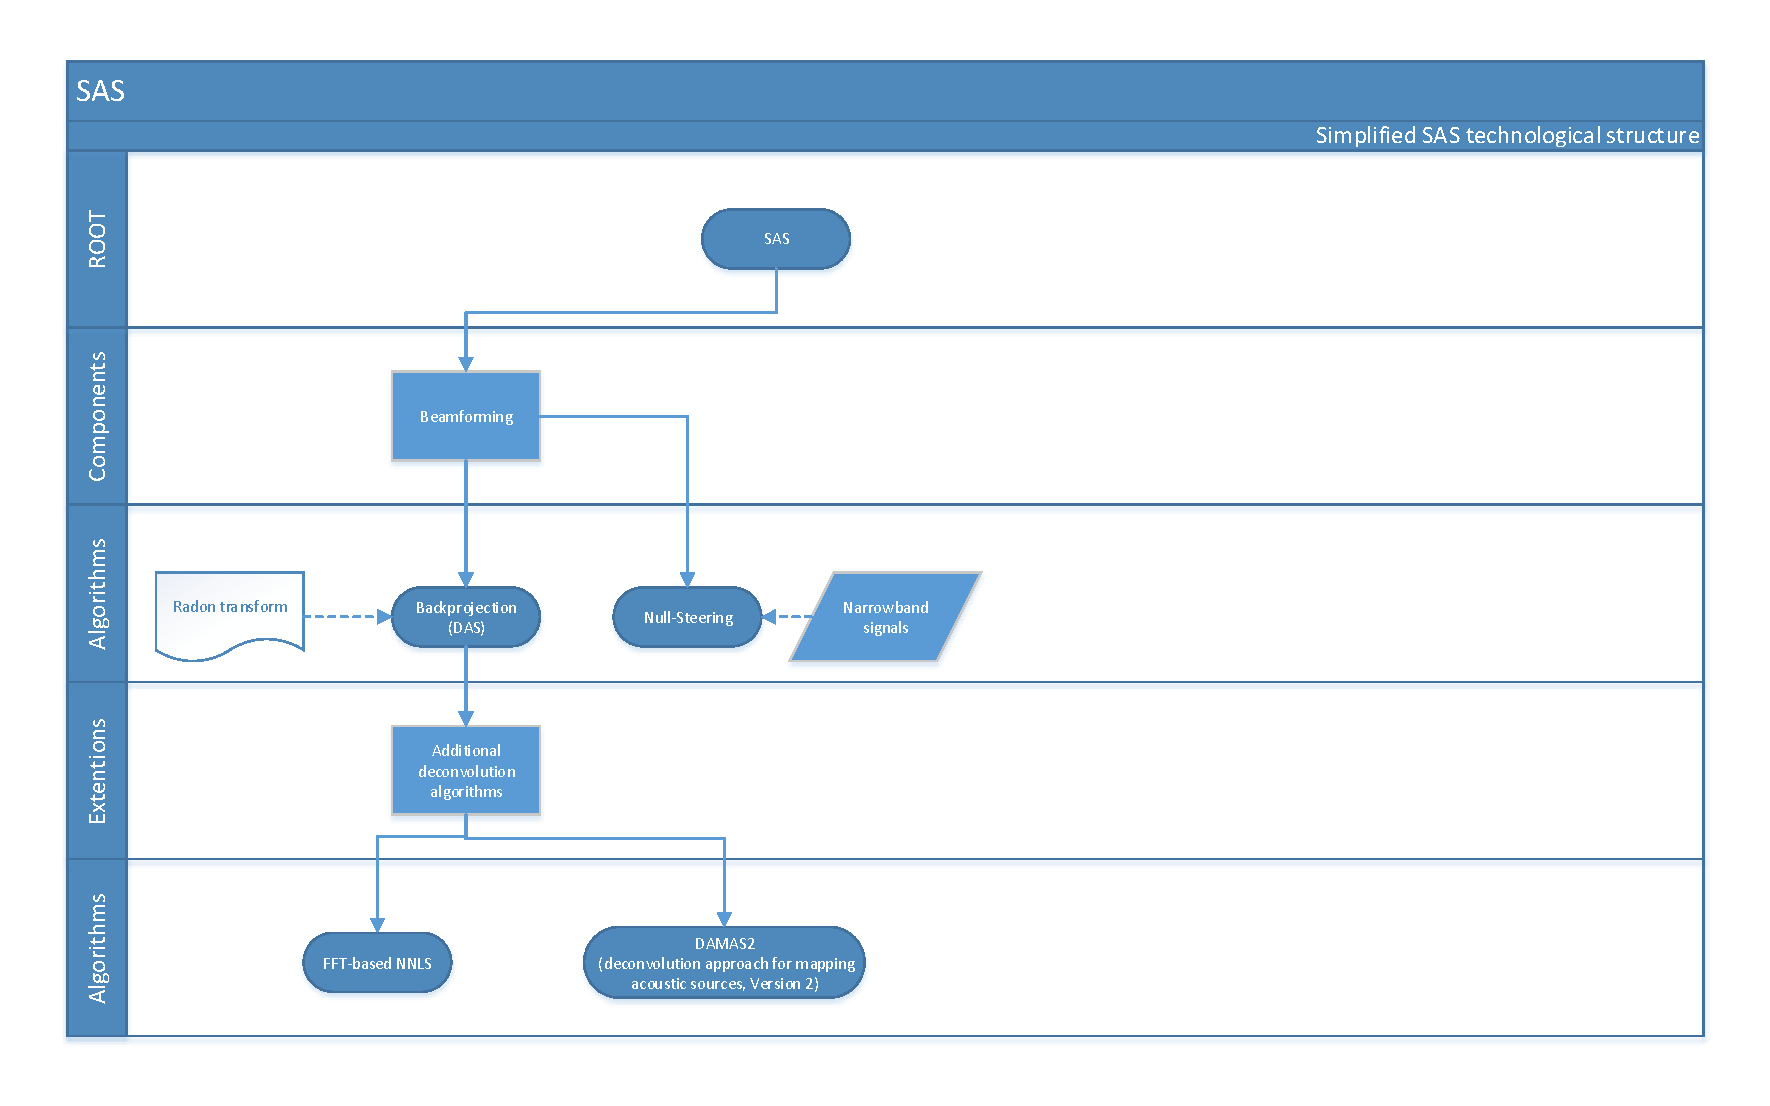
\includegraphics[width=\columnwidth]{SASvisio}
    \caption{Tecnologias utilizadas no SAS.} 
    \label{fig:sastech}
\end{figure} 



\bibliographystyle{coppe}
\bibliography{MapingSonar-SAS}

\end{document}



% $I(x,y)=K \phi (x,y) R(x,y) \cdot \frac{Z(x,y)-x\cdot
% \cpar{Z}{x}(x,y)}{\sqrt{x^2+Z^2(x,y)}\cdot
% \euTwo{\cpar{Z}{x}(x,y)}{\cpar{Z}{y}(x,y)}}$

%  \begin{figure}[H]
%     \centering
%     \includegraphics[width=0.4\columnwidth]{figs/forca/1.png}
%     \caption{Exemplo de um sensor de for�a: cilindro com strain gauge acoplado.}
%     \label{forca_1}
% \end{figure}